\documentclass[a0,portrait]{a0poster}
%\usepackage[spanish]{babel}
\usepackage[utf8]{inputenc}


\usepackage{times,colordvi,amsmath,epsfig,float,color,multicol}

\pagestyle{empty}
\setlength{\parindent}{0cm}
\setlength{\parskip}{2ex}
\setlength{\columnsep}{3cm}
\addtolength{\textwidth}{2cm}
\addtolength{\oddsidemargin}{-1.5cm}

\renewcommand{\normalsize}{\Large}
\def\regularsize{\@setfontsize\normalsize{34pt}{37}}

\renewcommand\refname{}
\setlength{\fboxrule}{0.1cm}


% ----------------------------------------------------------------


% PMS287 CMYK=[100% 69% 0% 11.5%] RGB=[38/256 67/256 151/256]
\definecolor{qmuldarkblue}{rgb}{0.1484375,0.26171875,0.58984375}

\definecolor{backgrey}{rgb}{0.93,0.93,0.93}
\definecolor{backblue}{rgb}{0.93,0.93,1}
\definecolor{backyellow}{rgb}{1,1,0.88}

\definecolor{backred}{rgb}{1,0.9,0.9}
\definecolor{backgreen}{rgb}{0.9,1,0.9}
\definecolor{backpink}{rgb}{1,0.9,1}
\definecolor{backturquoise}{rgb}{0.9,1,1}


\definecolor{backa}{rgb}{0.93, 0.8, 1}
\definecolor{backb}{rgb}{0.8, 0.93, 1}
\definecolor{backc}{rgb}{0.76, 0.82, 0.94}
\definecolor{backd}{rgb}{0.47, 0.65, 0.82}


% ----------------------------------------------------------------


\makeatletter
\renewcommand{\section}{\@startsection
        {section}                          % the name
        {1}                                % the level
        {0mm}                              % the indent
        {-0.7\baselineskip}                % the beforeskip
        {5mm}                              % the afterskip
        {\center\huge\color{qmuldarkblue}\bfseries}} % the style
\renewcommand{\subsection}{\@startsection
        {subsection}                          % the name
        {2}                                % the level
        {0mm}                              % the indent
        {-0.7\baselineskip}                % the beforeskip
        {5mm}                              % the afterskip
        {\center\Large\color{qmuldarkblue}\bfseries}} % the style

\makeatother


\usepackage{theorem}
{\theorembodyfont{\rmfamily}%
%\newtheorem{ejemplo}{Ejemplo}[section]}
%\usepackage{Sweave}

\begin{document}

%\vspace{1cm}

\colorbox{qmuldarkblue}{
 \color{white}
 
\begin{minipage}{0.2\textwidth}
\begin{center}
 \vskip 1cm
	
  
\includegraphics[width=8cm]{images/useRToulouse.png}
% Session Number \\ (\textit{t.b.a. by the organizers})   

%     \textit{	XXVIII International Biometric Conference}	Victoria, Canadà
     \end{center}
     
\end{minipage}


\begin{minipage}{0.6\textwidth}
\vspace*{0.4cm}
\begin{center}
   \textrm
   {
    {\huge \bf \em Lheuristic-A Shiny app to select genes potentially regulated by methylation}\\[1ex]
    {\large Sánchez-Pla, Alex$^{1,3}$, Castellano, Pol$^1$,  Mir\'{o}, Berta$^2$, Carmona, Francesc$^1$}\\[1ex]
    {\large $^1$ Departament of Genetics Microbiology and Statistics, Universitad de Barcelona\\
    $^2$ International Rice Research Institute, (IRRI), Philippines\\
    $^3$ Statistic and Bioinformatics Unit. Vall d'Hebron Research Institute.  (VHIR). Barcelona}
   }
   \end{center}
   
\vspace*{0.4cm}
\end{minipage}

\begin{minipage}{0.2\textwidth}
\begin{center}
   
\includegraphics[width=14cm]{images/allLogos.png}
   \end{center}
\end{minipage}
}
%\vspace{0.5cm}


% ----------------------------------------------------------------


\begin{multicols}{2}

\fcolorbox{black}{white}{\parbox{1.0\columnwidth}
{
\section{Introduction}

\begin{itemize}
\item Methylation %of CpG dinucleotides in the promoter 
of genes involved in the oncogenic process is a key process contributing to tumor initiation and/or progression\cite{sadikovic:2008}. 

\item Finding \textit{Genes Regulated by Methylation} or GRM can lead to a better understanding and be a guide to finding new drug targets.

\item This study originates in a work searching for colon cancer biomarkers \cite{bazzocco}. Cell lines with increasing sensitivity to a chemotherapy drug, were analyzed with Expression and Methylation arrays.  Finding GRM was used to search of candidate genes for new therapies.

\item In cancer--related genes it is common to observe a decrease in gene expression associated with hypermethylation. Methylation is often described as a binary on-off signal (\cite{Liu})
that is, when methylation is ``off'' the gene can express normally and
its expression will be low or high, whereas when methylation
is ``on'', the expression of the gene will be \emph{repressed} and its
values will tend to be low.

\item As a consequence of this \emph{high-methylation/low-expression} and
\emph{low-methylation/high-expression} relation plots depicting 
methylation and expression will show L--shape patterns so the
strategy adopted will be to mine such plots and select those that
have such a shape.

\end{itemize}

}}

\begin{center}
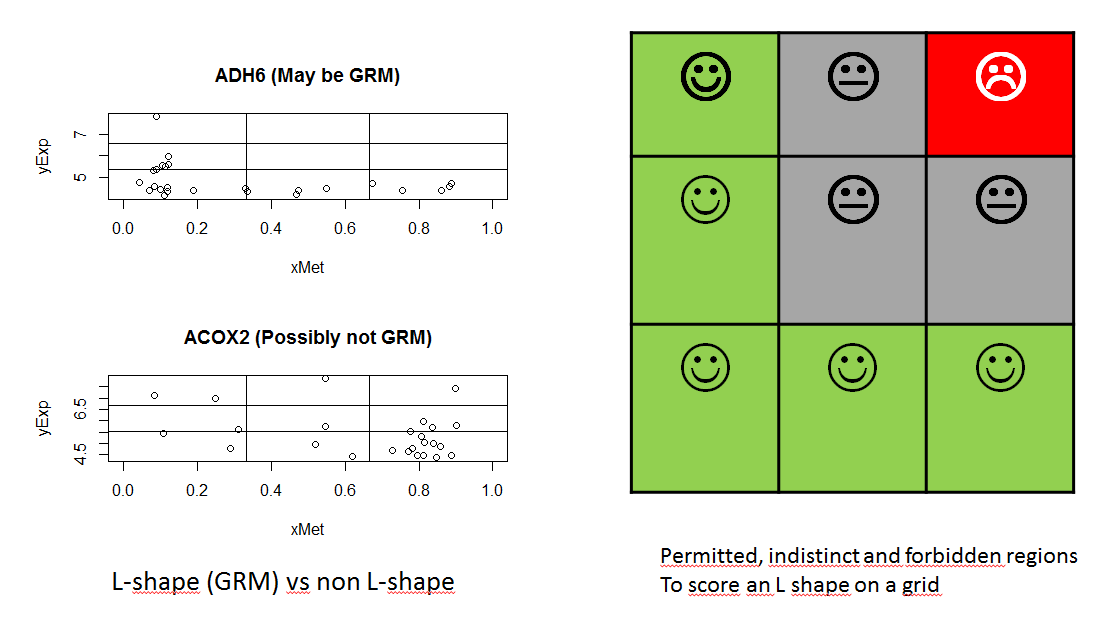
\includegraphics[width=0.9\columnwidth]{./images/Lshapes_1and2.png}
\end{center}

\fcolorbox{black}{backblue}{\parbox{1.0\columnwidth}
{\section{App Usage}

\begin{itemize}
 \item Data upload
  
\item Setting of parameters 

\item Analysis
  \begin{itemize}
    \item Method choice (Correlation, L-heuristic)
  \end{itemize} 
  
\item Intersection
  

\end{itemize} 


\begin{center}
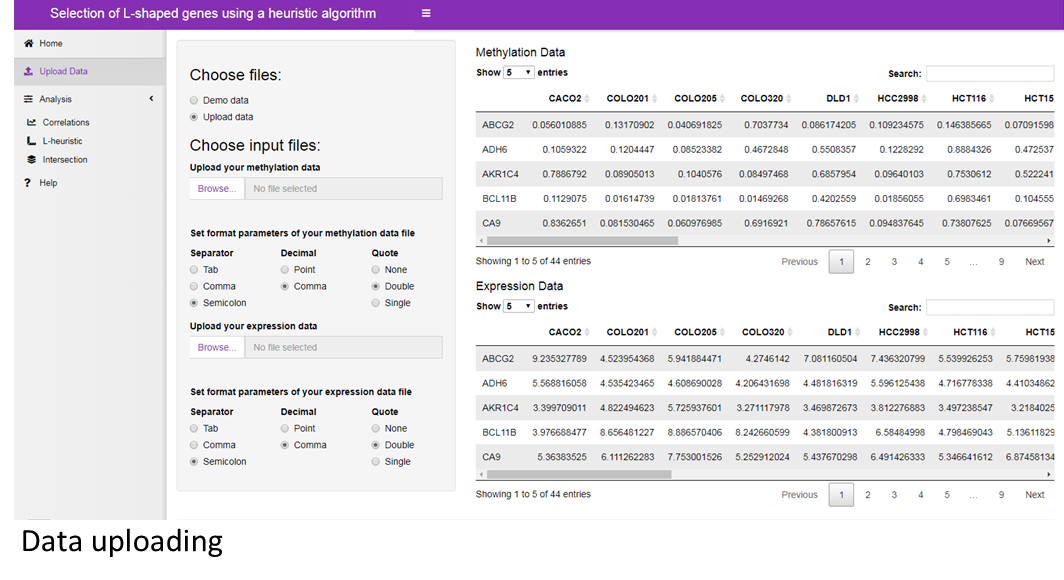
\includegraphics[width=0.9\columnwidth]{./images/data_uploading.png}
\end{center}}}

\vspace{0.1cm} 
\fcolorbox{black}{backgrey}{\parbox{1.0\columnwidth}
{\subsection{Correlation method}
a simple absolute correlation can be applied to the list of genes. The adjustable parameters are:

\begin{itemize}
\item Correlation type (Pearson, Spearman, Kendall)
\item Correlation coefficient
\item Correlation p-value
\end{itemize}

Optionally, a linear model fit can be overlayed on the scatterplot graph.

\begin{center}
	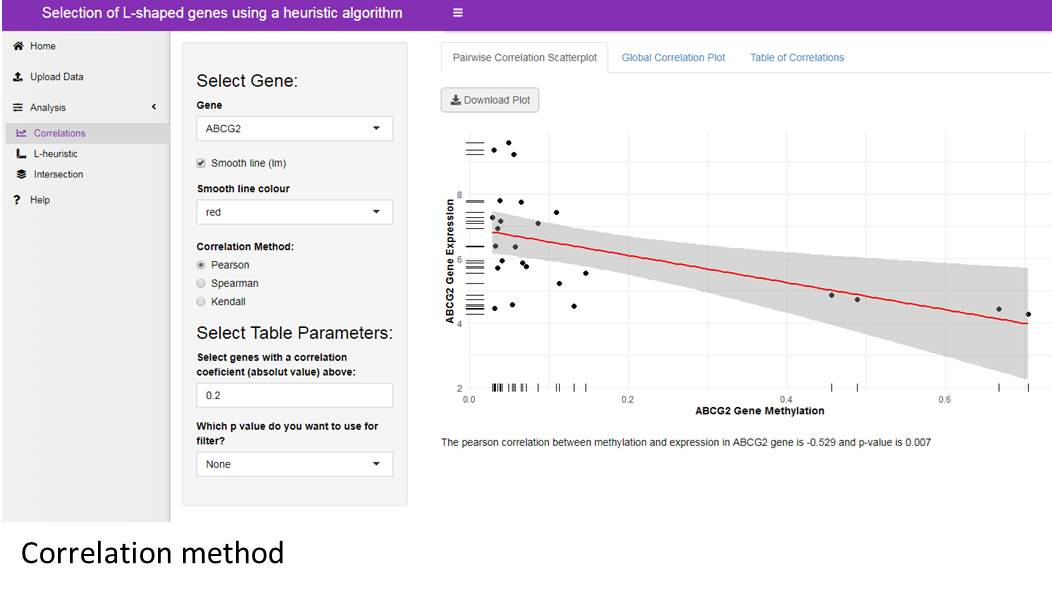
\includegraphics[width=0.8\columnwidth]{./images/correlation_method.png}
\end{center}

}}

%\vspace{0.6cm} 
\fcolorbox{black}{backgrey}{\parbox{1.0\columnwidth}
{\subsection{Intersection analysis}

A Venn diagram plots the relation of L-shaped genes selected between the correlation and the L-heuristic methods.

\begin{center}
	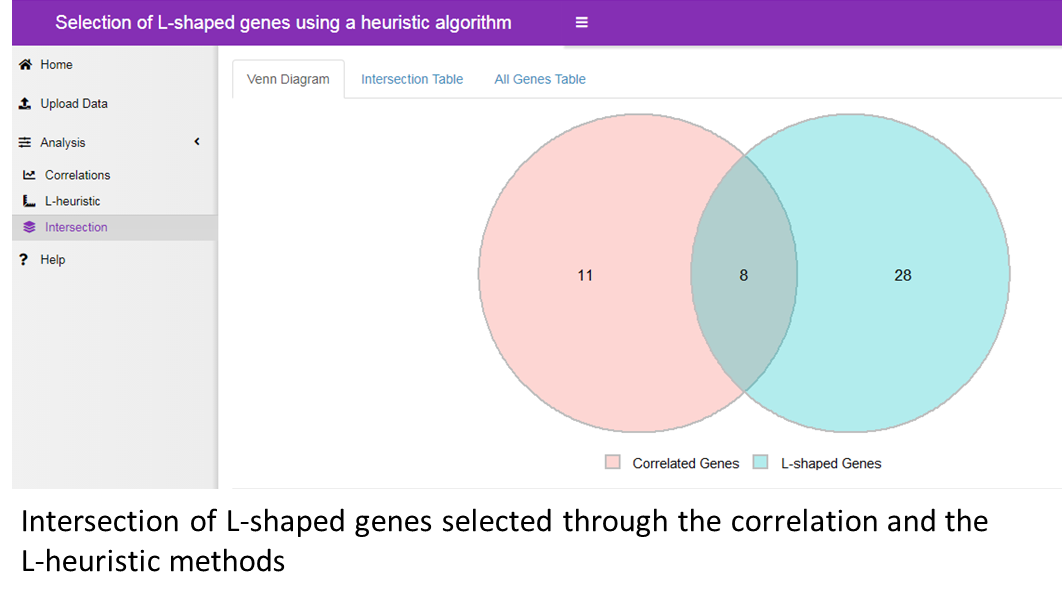
\includegraphics[width=0.8\columnwidth]{./images/intersection_method.png}
\end{center}
}}

\fcolorbox{black}{backgrey}{\parbox{1.0\columnwidth}
	{\section{What does the app do?}

Visually explore the realtion between expression and methylation -omic results to potentially identify genes regulated by methylation.

The app Lheuristic will:

\begin{itemize}
\item Two different methods of analysis
\item Step-by-step parameter selection
\item Instant data visualization
\item Table and graph export options and customization
\end{itemize}



}}

% \vspace{0.6cm}
\fcolorbox{black}{backyellow}{\parbox{1.0\columnwidth}
{\section{Results}
\begin{itemize}
	\item We developed a heuristic method based on imitating the visual selection of L-shapes by overimposing a $3\times 3$ grid on the scatterplot (\cite{sanchez:2019}).
	\item The algorithm has been implemented in R (package ready-to-be-submitted to Bioconductor).
	\item A Shiny application has been created to select genes potentially regulated by methylation using a combination of the \textit{Lheuristic} method and a naïve approach (negative correlation).
\end{itemize}
}}

%\vspace{1cm} \fcolorbox{black}{white}{\parbox{1.0\columnwidth}
%{\input{sectionsUseR/conc}}}

%\vspace{0.2cm} 
\small\vspace{-5mm}
\begin{thebibliography}{9}
%\addcontentsline{toc}{chapter}{\numberline{}Bibliografía}
%
%\bibitem{cohen} J. Cohen, \emph{Statistical power analysis for the behavioral sciences} (2nd ed.). % Hillsdale,NJ: Lawrence Erlbaum, 1988.

%\bibitem{faraway} J.J. Faraway, \emph{Linear Models with R}, Chapman \& Hall/CRC, 2004.

%\bibitem{montgomery} D.C Montgomery \emph{Design and Analysis of Experiments}, John Wiley \& Sons, 2008.

%\bibitem{blog} \texttt{http://erre-que-erre-paco.blogspot.com.es/2013/04/el-codigo-body-td-font-family-sans.html}

\bibitem{bazzocco} Sarah Bazzocco, Hafid Alazzouzi, M. Carme Ruiz de Villa, Alex Sanchez-Pla, John M. Mariadason, Diego Arango (2013) \emph{Genome-Wide Analysis of DNA Methylation in Colorectal Cancer}. Submitted.

\bibitem{Liu} Yihua Liu and Peng Qiu. (2012) \emph{Integrative analysis of methylation and gene expression data in TCGA} IEEE International Workshop on Genomic Signal Processing and Statistics (GENSIPS)

\bibitem{racine} Jeffrey Racine. (2012) A primer on regression splines.\newline
\verb|http://cran.r-project.org/web/packages/crs/vignettes/spline_primer.pdf|

\bibitem{sadikovic:2008}
B~Sadikovic, K~Al-Romaih, J.A Squire, and M~Zielenska.
\newblock {Cause and {Consequences} of {Genetic} and {Epigenetic} {Alterations}
	in {Human} {Cancer}}.
\newblock {\em Current Genomics}, 9(6):394--408, September 2008.

\bibitem{sanchez:2019}Sanchez-Pla, A., Mir\'o B., Carmona, F. et al.  \emph{A heuristic algorithm to select genes potentially regulated by methylation} [version 1; not peer reviewed]. F1000Research 2019, 8:1017 (slides) (doi: 10.7490/f1000research.1116986.1)

\end{thebibliography}
\normalsize

\end{multicols}


% ----------------------------------------------------------------

%\vspace{0.5cm}

\colorbox{qmuldarkblue}
{
 \color{white}
 \parbox{1.0\textwidth}
 {
 % \vspace{0.2cm}

{\small
	Work partially supported by research project MTM2015-64465-C2-1-R (MINECO/FEDER) from Ministerio de Economía y Competitividad and  by Grant 2014 SGR 464 (GRBIO) from the Departament d'Economia i Coneixement de la Generalitat de Catalunya.  
}%  \vspace{0.2cm}
 }
}


\end{document}
